\section{Results}\label{Sect_Results}
In this section we will analyse the results of all 3 model iterations. For the first two iterations we will show the prediction error on the ultimate for each \texttt{leaf} and province, while for the last iteration will will give the average monthly error. It should be noted that we only show the ultimate predictions for claims pending in 2017 and 2018, although we use the incurred as of March 2020. Pending claims in December 2018 had more than 14 months to develop to the ultimate. 
\subsection{First model iteration: Historical pending claims}
	\paragraph{Quebec:}
		For our first model, the average monthly prediction error is $957,758 \$$, based on a total volume of about 100 million. Figure \ref{Fig_QC_current_er_by_month} show that the error has a light seasonal pattern. In winter we tend to slightly underestimate, while in most months we overestimate the ultimate loss. The seasonality is difficult to confirm, since we only have 2 years of fully credible data. The error does not seem to be all random and thus should be further investigated. We do notice less cyclique pattern when using a lag and period length which includes the same month of the previous year. However, it does not neutralise it.
		\begin{figure}[H]
			\begin{center}
				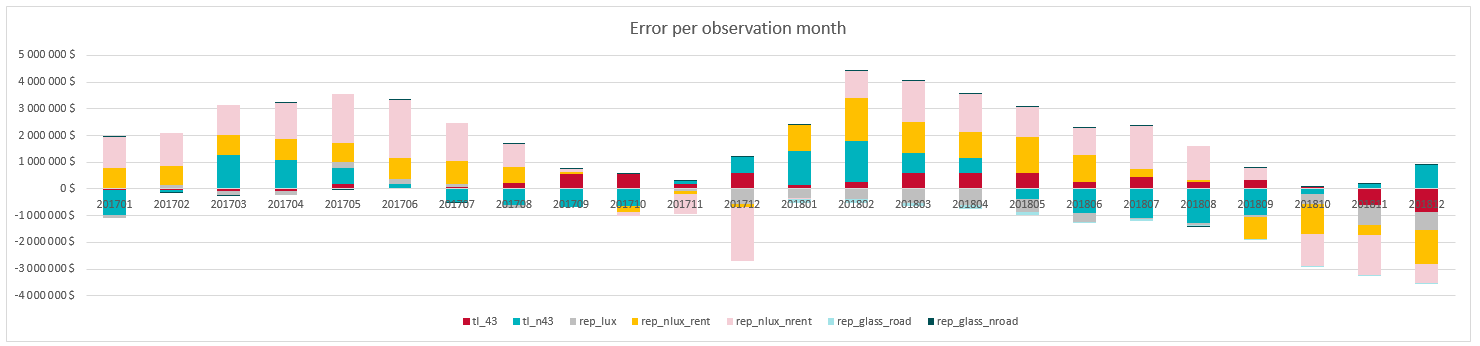
\includegraphics[scale=0.4]{Graphiques/QC_current_model_by_month} 
				\renewcommand{\figurename}{Figure}
				\caption{Quebec "Historical  pending claims" model, prediction error by observation month}\label{Fig_QC_current_er_by_month}
			\end{center}
		\end{figure}
		Figure \ref{Fig_QC_current_er_boxplot} indicates that the largest proportion of error comes form \texttt{tl\_n43} and \texttt{rep\_nlux\_nrent}.These two \texttt{leaf} are also the largest in terms of volume. 
		\begin{figure}[H]
			\begin{center}
				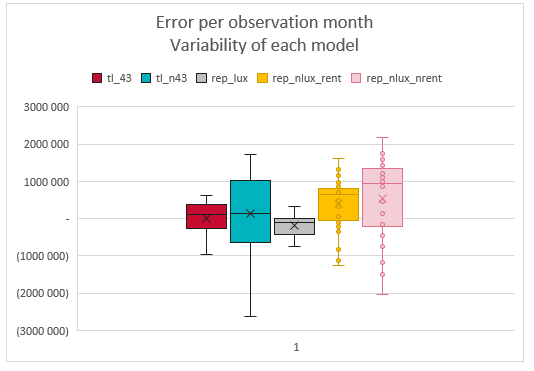
\includegraphics[scale=0.4]{Graphiques/QC_current_model_mustach} 
				\renewcommand{\figurename}{Figure}
				\caption{Quebec "Historical  pending claims" model, monthly prediction error boxplot}\label{Fig_QC_current_er_boxplot}
			\end{center}
		\end{figure}
	
	\paragraph{Ontario:}
		In Ontario, our model has the tendency to underestimate the ultimate amount. The average error per observation month shown in figure \ref{Fig_ON_current_er_by_month} is at $-4,632,282\$ $. Specifically, the winter proves difficult for our model. We are currently investigating this issue, but it might be related to the lag we use and/or the trends observed in the data.
		\begin{figure}[H]
			\begin{center}
				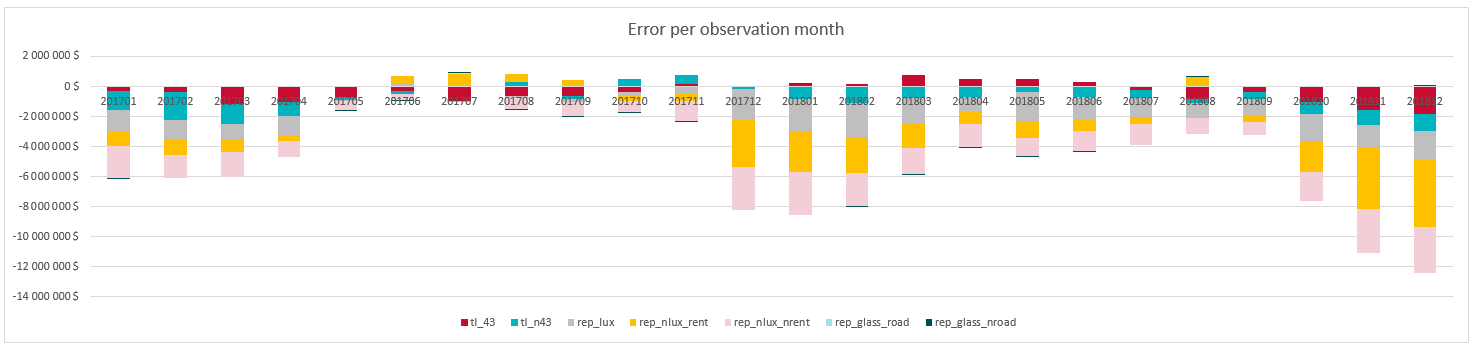
\includegraphics[scale=0.4]{Graphiques/ON_current_model_by_month} 
				\renewcommand{\figurename}{Figure}
				\caption{Ontario "Historical  pending claims" model, prediction error by observation month}\label{Fig_ON_current_er_by_month}
			\end{center}
		\end{figure}
		\begin{figure}[H]
			\begin{center}
				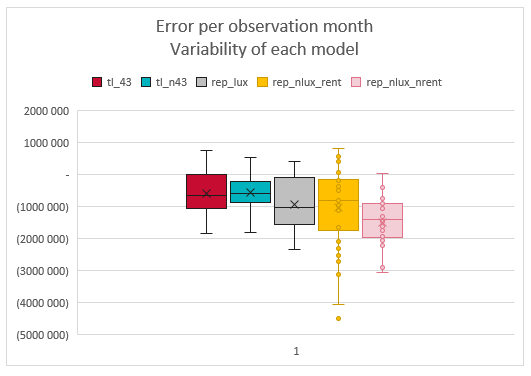
\includegraphics[scale=0.4]{Graphiques/ON_current_model_mustach} 
				\renewcommand{\figurename}{Figure}
				\caption{Ontario "Historical  pending claims" model, monthly prediction error boxplot}\label{Fig_ON_current_er_boxplot}
			\end{center}
		\end{figure}
	\paragraph{Alberta:}
		The average monthly prediction error amounts to $3,547,626\$ $ on a total volume of about 80 million. There is no clear seasonal pattern, however the model constantly overestimates. The cause of the overestimation is the subrogation, which even after 12 months is not completed. We found about 10\% of the claims in Alberta still receive recovery payments after 12 months. Figure \ref{Fig_AB_current_er_boxplot} shows that \texttt{rep\_nlux\_rent} is the biggest source of error for this model.   
		\begin{figure}[H]
			\begin{center}
				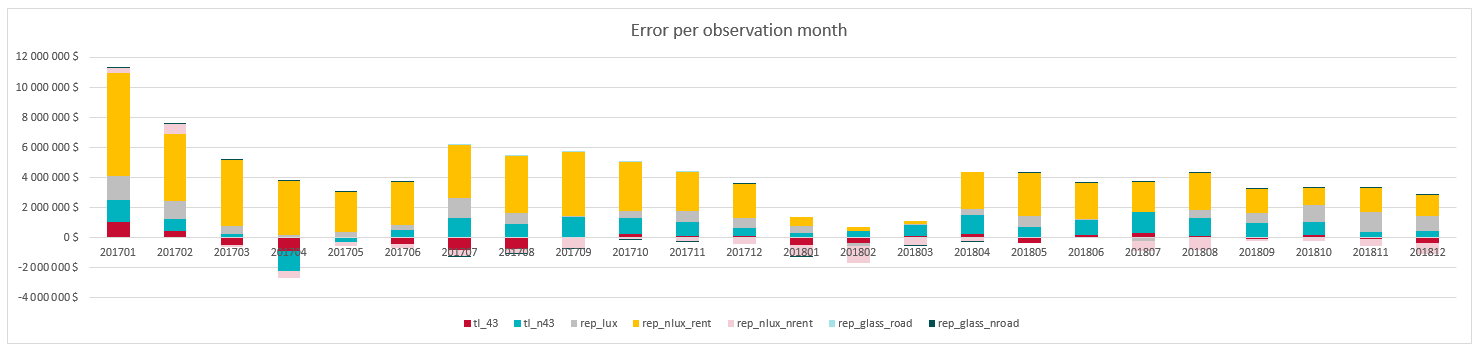
\includegraphics[scale=0.4]{Graphiques/AB_current_model_by_month} 
				\renewcommand{\figurename}{Figure}
				\caption{Alberta "Historical  pending claims" model, prediction error by observation month}\label{Fig_AB_current_er_by_month}
			\end{center}
		\end{figure}
		\begin{figure}[H]
			\begin{center}
				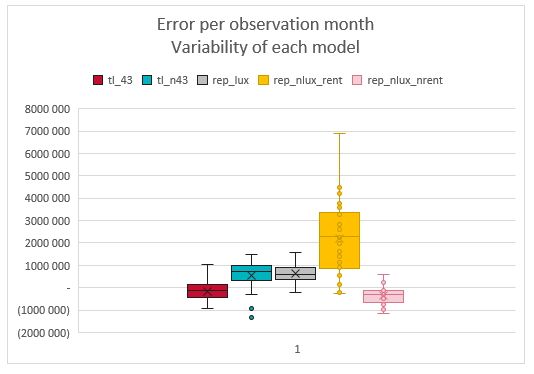
\includegraphics[scale=0.4]{Graphiques/AB_current_model_mustach} 
				\renewcommand{\figurename}{Figure}
				\caption{Alberta "Historical  pending claims" model, monthly prediction error boxplot}\label{Fig_AB_current_er_boxplot}
			\end{center}
		\end{figure}
	
	Overall, when combining all results we can observe that Onatrio and Alberta almost zero out. Figure \ref{Fig_IBNER_preds} shows our results for the December 2019 model (upper graph) and our current model (lower graph). Our current model is a sgnification improvement over the previous model. There error is rarely greater than 2 million \$. However, the red square indicates a zone of bad predictions amounting to error as high as 18 million \$. One should note that the real IBNER after February 2019 is not reliable, since it is not yet fully developed in some cases.
	
	\begin{figure}[H]
		\begin{center}
			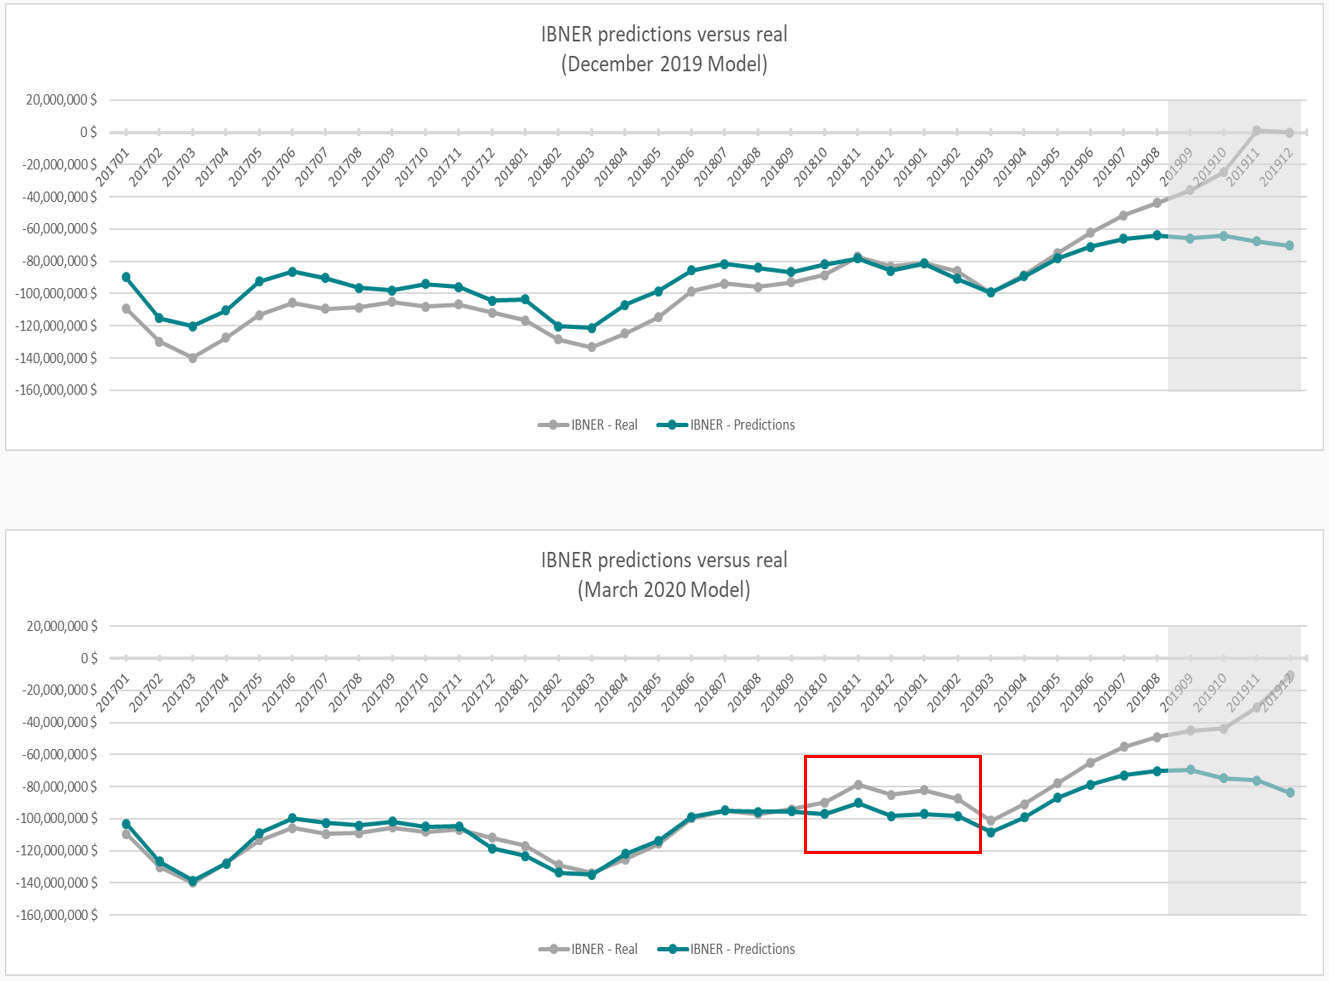
\includegraphics[scale=0.4]{Graphiques/JAN_vs_MARCH} 
			\renewcommand{\figurename}{Figure}
			\caption{IBNER prediction vs real IBNER}\label{Fig_IBNER_preds}
		\end{center}
	\end{figure}

\subsection{Second model iteration: Historical pending but now closed claims}
	Excluding open claims in the factor calculations has a strong impact on the model. The average monthly error are $-1,379,997 \$ $, $-5,134,386 \$ $ and $-431,989\$ $, for Quebec, Ontario and Alberta respectively. This model has a strong tendency to underestimate. Albeit, for Alberta, when looking at figure \ref{Fig_AB_closedonly_er_by_month}, the results are considerably better than the first iteration model. Adding open claims seems to multiply the error by a factor of 10. This indicated that once a claim is closed, the subrogation process seems to also be finished or partly finished. For the other two provinces, it shows that adding open claims captures something we are not yet able to fully explain. We suspect that the issue is related to the imputation method and observed trends.
		\begin{figure}[H]
			\begin{center}
				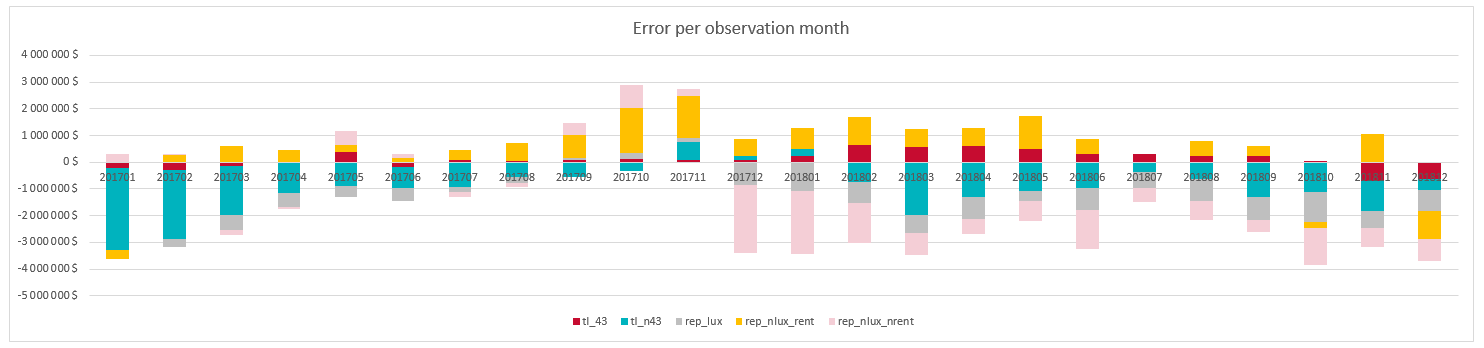
\includegraphics[scale=0.4]{Graphiques/QC_closedonly_model_by_month} 
				\renewcommand{\figurename}{Figure}
				\caption{Quebec "Historical  pending but now closed claims" model, prediction error by observation month}\label{Fig_QC_closedonly_er_by_month}
			\end{center}
		\end{figure}
		\begin{figure}[H]
			\begin{center}
				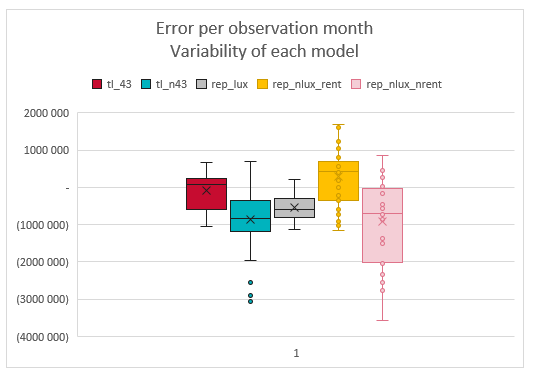
\includegraphics[scale=0.4]{Graphiques/QC_closedonly_model_mustach} 
				\renewcommand{\figurename}{Figure}
				\caption{Quebec "Historical  pending but now closed claims" model, monthly prediction error boxplot}\label{Fig_QC_closedonly_er_boxplot}
			\end{center}
		\end{figure}

		\begin{figure}[H]
			\begin{center}
				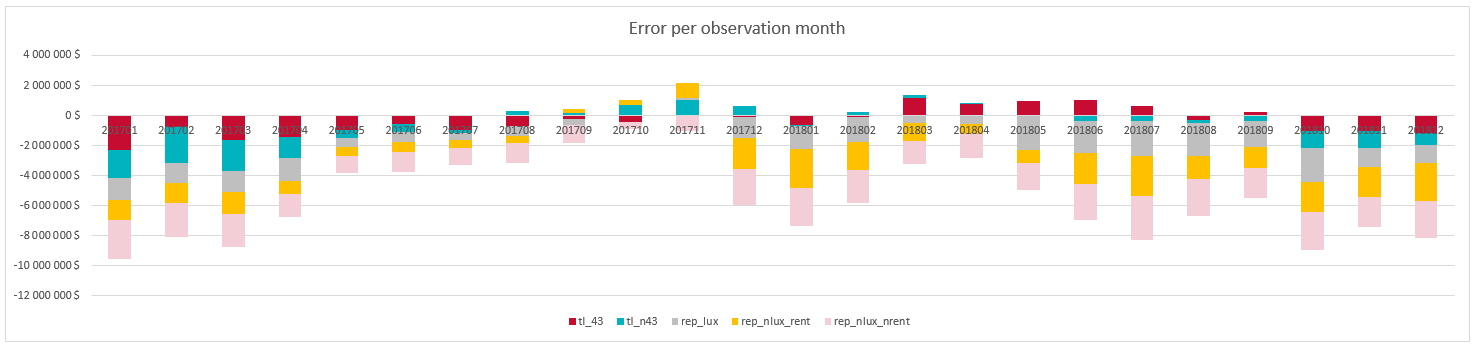
\includegraphics[scale=0.4]{Graphiques/ON_closedonly_model_by_month} 
				\renewcommand{\figurename}{Figure}
				\caption{Ontario "Historical  pending but now closed claims" model, prediction error by observation month}\label{Fig_ON_closedonly_er_by_month}
			\end{center}
		\end{figure}
		\begin{figure}[H]
			\begin{center}
				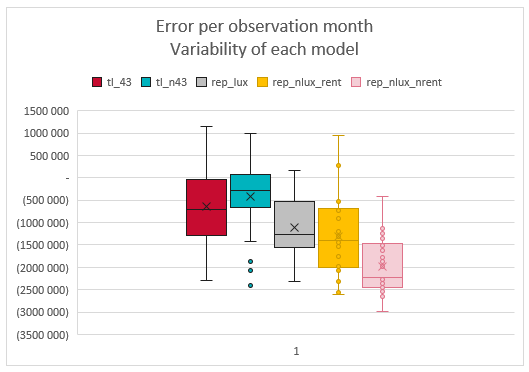
\includegraphics[scale=0.4]{Graphiques/ON_closedonly_model_mustach} 
				\renewcommand{\figurename}{Figure}
				\caption{Ontario "Historical  pending but now closed claims" model, monthly prediction error boxplot}\label{Fig_ON_closedonly_er_boxplot}
			\end{center}
		\end{figure}


		\begin{figure}[H]
			\begin{center}
				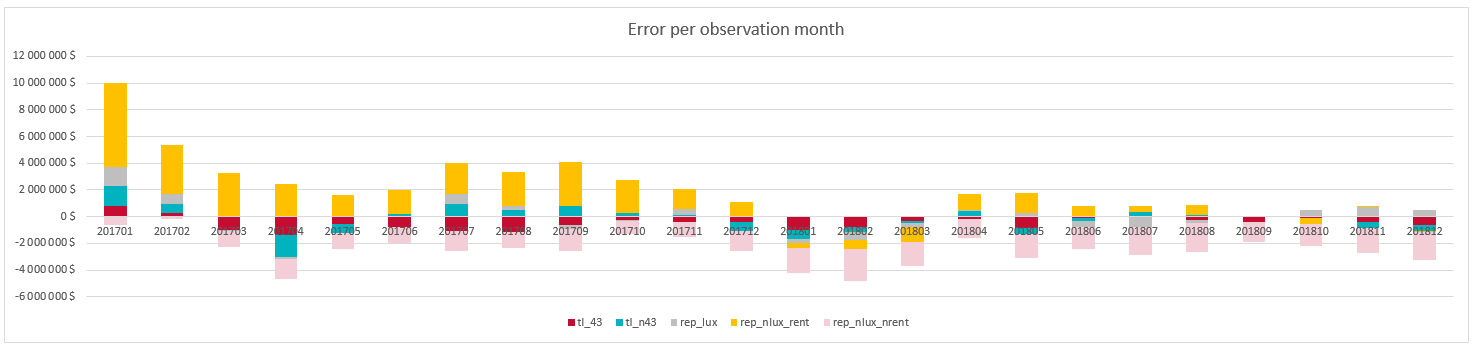
\includegraphics[scale=0.4]{Graphiques/AB_closedonly_model_by_month} 
				\renewcommand{\figurename}{Figure}
				\caption{Alberta "Historical  pending but now closed claims" model, prediction error by observation month}\label{Fig_AB_closedonly_er_by_month}
			\end{center}
		\end{figure}
		\begin{figure}[H]
			\begin{center}
				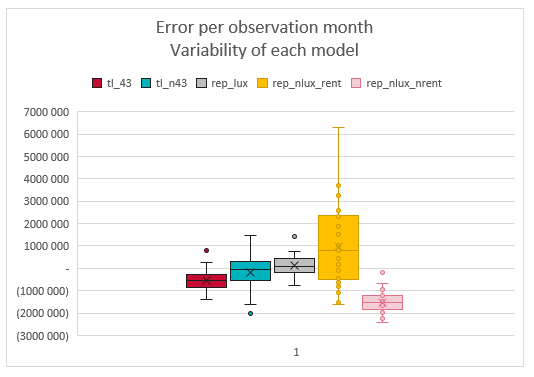
\includegraphics[scale=0.4]{Graphiques/AB_closedonly_model_mustach} 
				\renewcommand{\figurename}{Figure}
				\caption{Alberta "Historical  pending but now closed claims" model, monthly prediction error boxplot}\label{Fig_AB_closedonly_er_boxplot}
			\end{center}
		\end{figure}
	
\subsection{Third model iteration: Historical closed claims }
	Lastly, the third iteration model seems not to function as well as expected. Quebec has an average monthly error of $-7,196,717 \$ $, Ontario of $-13,153,106 \$ $ and Alberta of $4,148,104 \$ $. One issue with this model is related to the claims in the window. While the two previous model use a small window of pending claims, this model uses all claims that closed in the time window. Thus, we are using claims that can be very old relative to the observation month. Therefore the age of a claim might have a considerable impact on this model.
	
	
		 